\documentclass[review]{elsarticle}
\usepackage{lineno,hyperref}
\usepackage{subcaption}
\usepackage{siunitx}
\usepackage{booktabs}
\usepackage{graphicx}
\usepackage{appendix}
\usepackage{amsmath} 
\usepackage[hang,flushmargin]{footmisc} 
\usepackage{xcolor}
\usepackage{float}
\usepackage{array,multirow}
\usepackage{hyperref}
\usepackage{setspace}
\usepackage{stmaryrd}
\usepackage{enumitem}
\usepackage{rotating}
\usepackage{adjustbox}
\usepackage{array}
\usepackage{booktabs}
\usepackage{xcolor,colortbl}
\usepackage{amsmath} 
\usepackage{amsfonts} 
\usepackage{amssymb}
\usepackage{makecell}
\usepackage{amsmath}
\usepackage{nicefrac}
\usepackage{todonotes}
\usepackage{multirow}
\modulolinenumbers[1]
\usepackage{lineno}
\usepackage{tikz}

%\usepackage[final]{changes}
\usepackage{changes}
\usepackage[ruled,vlined,linesnumbered,lined,boxed,commentsnumbered]{algorithm2e}
\newcommand\mycommfont[1]{\footnotesize\ttfamily\textcolor{blue}{#1}}
\SetCommentSty{mycommfont}
\newcommand{\BREAK}{\STATE \algorithmicbreak}
\modulolinenumbers[1]
\setlength{\parindent}{0em}
\journal{Applied Energy}
\bibliographystyle{elsarticle-num}

\begin{document}
\begin{frontmatter}

%\title{Justice in decarbonizing heating systems consistent with the Paris Climate Agreement: subsidy balance between landlords and tenants at the multi-apartment building level}
\title{Equitable decarbonization of the heat supply of rented residential buildings: Optimal subsidization strategy under allocating the costs of inaction}
\author[1]{Sebastian Zwickl-Bernhard\corref{cor1}}
\ead{zwickl@eeg.tuwien.ac.at}
\author[1]{Hans Auer}
\author[1]{Antonia Golab}
\cortext[cor1]{Corresponding author}
\address[1]{Energy Economics Group (EEG), Technische Universität Wien, Gusshausstrasse 25-29/E370-3, 1040 Wien, Austria}

\begin{abstract}

\end{abstract}

\begin{keyword}
	
\end{keyword}
\end{frontmatter}

\newpage
\section*{Nomenclature}
\begin{center}
	\renewcommand{\arraystretch}{1.1}
	\centering
	\small
	\begin{tabular}{lm{8cm}r}
		Type & Description & Unit\\
		\hline
		Set and index & & \\
		\hline
		
		{$y \in \mathcal{Y}=\{1,\ldots,Y\}$} & Years, index by $y$\\
		{$m \in \mathcal{M}=\{1,\ldots,M\}$} & Months, index by $m$\\
		
		\hline
		Decision variables\\
		\hline
		{$\Psi$} & Investment grant paid to the landlord & \SI{}{EUR}\\
		{$\Omega_{y,m}$} & Heating costs subsidy payment for a single tenant in $y$ and $m$ & \SI{}{EUR}\\
		{$d_{y,m}$} & Total heat demand per dwelling & \SI{}{kWh}\\
		{$q_{y,m}$} & Heat demand supplied by the heating system alternative & \SI{}{kWh}\\
		{$\pi$} & Newly installed heating system alternative capacity & \SI{}{kW}\\
		{$r_{y,m}$} & Rent charge adjustment in $y$ and $m$ & \SI{}{EUR\per m^2}\\
		\hline
		Relevant parameters\\
		\hline
		{$n$} & Number of tenants within the multi-apartment building & \SI{}{1}\\
		{$i$} & Interest rate & \SI{}{\%}\\
		{$q_{load,y,m}$} & Total heat demand in $y$ and $m$ & \SI{}{kWh}\\
		{$\alpha_{m}$} & Monthly load factor (ratio between total and peak heat demand) in $m$ & \SI{}{1}\\
		{$c_{alt}$} & Specific heating system alternative investment costs & \SI{}{EUR \per kW}\\
		{$c_{con}$} & Heating system alternative construction costs & \SI{}{EUR}\\
		{$\bar{r}$} & Initial rent price & \SI{}{EUR \per m^2}\\
		{$\rho$} & Upper bound of the biannual rent charge adjustment & \SI{}{\%}\\
		{$a$} & Rented area per tenant/dwelling & \SI{}{m^2}\\
		{$p_{init,y}$} & Energy price fueling the initial heating system & \SI{}{EUR \per kWh}\\
		{$p_{alt,y,m}$} & Energy price fueling the heating system alternative & \SI{}{EUR \per kWh}\\
		\hline
	\end{tabular}
\end{center}
\newpage

\section{Introduction}
The recently published "Fit for 55" package \cite{european_commission_european_2019} by the European Commission outlines the pathway until 2030 to reduce greenhouse gas emissions by \SI{55}{\%} compared to 1990 in the Europe Union (EU). With an eye on the therein described energy policy recommendations, undisputedly, massive efforts across sectors are necessary to enable a sustainable transformation of the energy system (see also in \cite{korkmaz2020comparison}). At the same time, there is a need for energy justice complying with the manner of "no one left behind" \cite{sovacool2019decarbonization}. Against this background, the residential building sector calls for particular attention. There are at least three reasons for this: (i) High shares of fossil fuels in the provision of heat service needs (but also the cold service needs as well), (ii) Inefficient ways of delivering the heat demand caused by low standards in terms of building stock quality and heat generation technologies, (iii) Complex building ownership structures and the fact that many people do not live in a property but in rented apartments or dwellings.\vspace{0.5cm}

In fact, buildings are responsible for \SI{40}{\%} of EU energy consumption and \SI{36}{\%} of the greenhouse gas emissions. Moreover, the European Commission states that \SI{75}{\%} of EU's buildings are energy efficient. The essential factor to improve these indicators is building retrofitting. Passive renovation measures can already make a significant contribution, as \SI{35}{\%} of EU's buildings are older than \SI{50}{} years. However, this alone will not bring the European building stock to deep decarbonization. Rather, it is necessary to increase the current renovation rate of \SI{1}{\% \per year} \cite{eurocombuildings2021}. Thus, the share of passive (e.g., insulation improvements) alongside active renovation (e.g., heating system change) measures needs to be increased rapidly to be compliant with European climate plans such as the abovementioned Fit for 55 package. Indeed, European decarbonization scenarios assume a much higher renovation rate up to \SI{3}{\%} in order to achieve climate neutrality \cite{korkmaz2020comparison}. To increase this rate, most scientific literature findings suggest federal financial incentives since renovation measures do not achieve economic viability under current market environments in the EU (see, e.g., Fina et al. \cite{fina2019profitability}, Weber and Wolff \cite{weber2018energy}, and Kumbaroğlu and Madlener \cite{kumbarouglu2012evaluation}).\vspace{0.5cm}

We have already seen in the last decades how federal financial incentives have led to massive market penetration of renewable energy technologies. For example, solar photovoltaic (PV) has flooded the electricity markets driven by public monetary subsidies such as feed-in tariff programs \cite{hoppmann2014compulsive}. In addition, significant cost reductions were found due to efficiency improvements and economies of scale \cite{haas2011historical}. In principle, there are good reasons to think that one can learn from the diffusion pathway of solar PV and related experiences. Nevertheless, two aspects are crucial in this context that has received too little attention in the past. First that the public monetary diffusion of renewable energy has to be accompanied by measures ensuring energy efficiency. Recently, Poponi et al. \cite{poponi2021subsidisation} conducted a subsidization cost analysis of renewable energy deployment in Italy. Studying the diffusion of solar PV, they concluded that public monetary support strategies are a cost-ineffective policy instrument if energy efficiency investments are ignored. And second, that the support needs to be socially balanced in terms of society with and without private ownership, which is essential for many renewable technology investments, not only in the heating sector.\vspace{0.5cm}

The scope of this paper aims at exploring one "hot potato" of a sustainable society future, namely, the decarbonization of the rented residential building sector in terms of heating system change and passive retrofitting measures. A focus lies on multi-apartment buildings in urban areas that are often heated by natural gas-based heating systems. Moreover, the frequently occurring ownership structure within the building with a single landlord (building owner) and numerous tenants plays a key role in the analysis as this is a generally crucial relationship since typically, a building's landlord is the decision-maker in terms of potential (active and passive) retrofitting measures but is not influenced by an increasing CO\textsubscript{2}, as the key determining parameter of deep decarbonization strategies in its decision process yet. On the contrary, the tenants are impacted significantly by the CO\textsubscript{2} price but without ownership, not able to invest in sustainable heat supply measures independently.\vspace{0.5cm}

Against this background, the core objective of this work is to determine a cost-optimal and socially balanced subsidization strategy for a multi-apartment building to trigger a sustainable heat supply. The governance incentivizes the replacement of the initial natural gas-based heating system toward a sustainable alternative along with building renovation measures to increase efficiency and reduce heat demand by monetary support to the landlord and the tenants. Federal subsidy payments can be direct payments in the form of an investment grant for the landlord or a subsidy payment for the tenant. Besides, the owner can also be indirectly financially supported by allowing a rent adjustment as the building is refurbished. Social balance is defined at the building level from a monetary perspective using the net present value of the governance's subsidy payments for the building's owner and the tenants. This is also associated with a significant increase in the efficiency of the heat supply by passive retrofitting measures.\vspace{0.5cm}

The method applied is the development of a linear optimization model. Thereby, the objective function is to minimize the governance's net present value. The landlord's and tenants' strategy to minimize total costs in considered by tailor-made adapted constraints in the modeling framework. The generalized formulation of the model allows to investigate different building types and categorizes (e.g., size and number of tenants, building's efficiency, initial rent price, etc.) that can be helpful to represent different building stocks.\vspace{0.5cm}

The numerical example analyzed is a multi-apartment old building with a single owner and 30 units or tenants respectively. The partially renovated building is located in an urban area and initially heated by individual gas heating systems at the unit's level. The decarbonization of the heat supply can be achieved by two different options, namely, a connection to the district heating network or an implementation of an air-sourced heat pump system.\vspace{0.5cm}

The paper is organized as follows. Section \ref{stateoftheart} summarizes the current state-of-the-art in research and outlines the present study’s own contribution beyond the existing literature. Section \ref{methodology} presents the materials and methods developed in this work including the mathematical formulation of the model, scenario and numerical example description and model validation. Section \ref{results} presents the results of this work, including sensitivity analyses of key determining parameters. Section \ref{conclusions} discusses the results, concludes the work, and outlines possible future research.
\newpage
\section{State-of-the-art and progress beyond}\label{stateoftheart}
This section aims to provide an overview of relevant scientific contributions with respect to this paper's scope. Explicitly not part of the literature review is the already widely discussed topic of sharing renewable energy generation and related peer-to-peer innovations in the light of energy communities. A general study comprehensively dealing with the sharing economy is provided by Codagnone and Martens \cite{codagnone2016scoping}. The reviews from Sousa et al. \cite{sousa2019peer} and Koirala et al. \cite{koirala2016energetic} go into even more depth and with resepect to peer-to-peer energy sharing and energy communities. Also the authors' literature review of this paper in \cite{zwickl2021open} provides a comprehensive review of energy sharing on the local level.\vspace{0.5cm}

Against this background, the focus here lies on three different dimensions without claiming to be absolutely complete in each case. The first dimension is the decarbonization of heating and cooling systems from a system analysis perspective and is described in Section \ref{aspect1}. The second dimension deals with the increasingly importance of justice in the energy system transition and is presented in Section \ref{aspect2}. The third dimension is dedicated to the trade-offs analysis of investment decisions into renewable energy technologies including realted contracting business cases and is discussed in Section \ref{aspect3}. The choice of these focal points, as well as the explicit exclusion of the mentioned topics, are deliberately chosen in order to reflect the DNA of the analysis. 

\subsection{Decarbonizing the provision of heating service needs}\label{aspect1}
The insights obtained from various scientific studies allow us to see the big picture of a decarbonized heating and cooling sector. A fundamental change of the energy carrier mix, alongside a significant efficiency increase, is necessary for a sustainable heating and cooling service need supply. For example, Connolly et al. \cite{connolly2014heat} provide in their study such a strategy and present a decarbonization roadmap for the European heating sector. They propose a new sustainable heat strategy that is based on changes on the demand-side and supply-side. In addition to significant heat savings, integrating sustainable heat sources into centralized heat networks (or district heating networks) and electrifying heat supply (e.g., heat pump) are suggested to achieve a low-carbon heating sector. Seyboth et al. \cite{seyboth2008recognising} focus in their study on supportive energy policy recommendations to enhance the deployment of renewable energy heating and cooling technologies. In particular, this means the integration of renewable sources such as solar, geothermal, and biomass into heating and cooling systems.\vspace{0.5cm}

In general, the sustainable heat source or heat generation technology that is ultimately implemented/used at the end-user levels depends on a number of factors. Among these, geographical and spatial characteristics (e.g., availability of heat network infrastructure, building construction features, outdoor temperature, etc.), in particular, play a crucial role. Su et al. \cite{su2018heating} deal in their study with optimal sustainable heating system alternatives with a special focus on local geographical features of the application site. Their results show that there might not be a one-fits-all solution if decarbonizing local heating systems. However, certain trends are very much emerging in their findings, which can also be confirmed by further case studies. Renewable-fed district heating networks have significant potential to supply heat demand in urban areas. This is exemplarily also shown by the results of Popovski et al. \cite{popovski2018technical}. They state that from a socio-economic perspective, district heating networks with excess heat are the most favorable supply option in densely populated areas. Lake et al. \cite{lake2017review} present a comprehensive review of district heating and cooling systems. They analyze among others the economic feasibility and system identification based on primary energy sources of centralized heating and cooling networks. Rama et al. \cite{rama2018introduction} study the optimal combination of different sustainable heating alternatives.In particular, they show how heat pumps and solarthermal can assist district heating networks. There exist also other alternatives. Sopha et al. \cite{sopha2011exploring} focus in their study on the potential of wood-pellet in Norway, a country with high shares of district heating-based heat supply. They use an agent-based model to identify energy policy options supporting the uptake of such sustainable heating systems. The authors conclude that a stable financial support (i.e., stable wood-pellet price) has the highest impact on the transition of wood-pellet. We refer to Section \ref{aspect3} in this context for a detailed discussion of financial incentives for renewable energy technologies in the heating sector.\vspace{0.5cm}

In any case, there is a need for sustainable alternatives to district heating. Either to complement existing district heating networks in a high-efficient way (e.g., \cite{rama2018introduction} and \cite{sopha2011exploring}) and/or because to compensate non-existing networks in the future. Popovski et al. \cite{popovski2018technical} identify the electrification of the heat supply using heat pumps with photovoltaics as the most cost-competitive alternative from a socio-economic perspective. Leibowicz et al. \cite{leibowicz2018optimal} also show end-use electrification as an optimal strategy for the decarbonization of the heating sector. However, the authors state that the electrification using heat pumps for example only makes sense in combination with building thermal efficiency improvements.\vspace{0.5cm}

In order to emphasize the importance of building renovation measures, we dedicate this concluding paragraph the corresponding literature. In particular, we select papers focusing on the impact of different retorfitting measures on sustainable heating system alternatives. However, we do not differentiate here in detail between different types of retrofitting measures (e.g., purely passive, passive, active, etc.) and refer in this context to the comprehensive literature review of Fina et al. in \cite{fina2019profitability}. Ma et al. \cite{ma2012existing} provide an extensive literature and state-of-the-art analysis of retrofitting focusing on existing buildings. Vieites et al. \cite{vieites2015european} elaborate in this context of European initiatives improving  the energy efficiency in existing and old (historic) buildings. Recently, Weinberger et al. \cite{weinberger2021investigating} investigate the impact of retrofitting on district heating networks. Fina et al. \cite{fina2019profitability} put their focus on the profitability of retrofitting of multi-apartment buildings with special consideration of different heating systems. They thoroughly study the implementation of the combination of building-attached/integrated photovoltaics supporting sustainable heating systems. Their results show how (passive) retrofitting measures result in a reduction of the required installed heating system capacity. However, the energy cost reduction achieved from higher building standards are not able to compensate the initial passive renovation investment costs. They conclude that latter significantly depend on the development of the CO\textsubscript{2} price and the assumptions of end-user investment grants as well as subsidies. We again take up these findings associated with financial support in Section \ref{aspect3}

\subsection{Justice in energy systems: fair and socially balanced sustainable energy transition}\label{aspect2}
The issue of justice in energy systems is addressed in various studies. According to them, a key part of achieving climate targets is to ensure that no one is left behind in the climate action. More generally, the three energy justice tenets are distributive, recognition, and procedural\footnote{In some works, restorative and cosmopolitan justice are also mentioned in this context. See, exemplarily in \cite{oxfordjustice2021}.}. Recently, these are comprehensively discussed and reviewed by Pellegrini et al. \cite{pellegrini2020energy}. Considering this work's scope, we put our focus on procedural justice, as it represents measures that reduce potential barriers to new clean energy investments \cite{oxfordjustice2021}.\vspace{0.5cm}

Generally speaking, dealing with just sustainable energy systems is a monumental task and seems to be very challenging to be generalized. However, studies focusing on certain local regions are likely to be the most promising approach. Recently, van Bommel and Höffken conducted a review study focusing on energy justice at the European community level \cite{van2021energy}. Besides that, Lacey-Barnacle et al. \cite{lacey2020energy} focus in their study on energy justice in developing countries. Coming back to this paper's content and spatial scope, Mundaca et al. \cite{mundaca2018successful} propose two local European case studies in Germany and Denmark investigating local energy transition from an energy justice perspective. Their findings are in line with those from Jenkins et al. \cite{jenkins2018humanizing} showing that energy justice and transitions framework can be combined and achieved simultaneously. However, Hiteva and Soacool \cite{hiteva2017harnessing} conclude from a business model perspective that energy justice may be realized through market principles but not through the market alone. We continue discussing this point in Section \ref{aspect3} when dealing with necessary (financial) incentives that foster the sustainable energy transition. \vspace{0.5cm} 

Recently, Hanke et al. \cite{hanke2021renewable} investigate renewable energy communities and their capability to deliver energy justice. They explore insights from 71 European cases and highlight the necessity of distributing affordable energy to vulnerable households. Furthermore, it is necessary to focus in this regard on low-income households. Exemplarily, Xu and Chen \cite{xu2019energy} propose on the basis of their generated results that low-income households need tailored assistance to ensure energy justice. In particular, they demonstrate that low-income households are renters and thus have fewer energy efficiency appliances. Sovacool et al. \cite{sovacool2019temporality} heat in the same direction and discuss the special difficulties for households without the capital for sustainable energy investments and for those that do not own their own home such as renters. Moreover, renters also often have higher residential heating energy use intensity, an energy efficiency proxy \cite{reames2016targeting}. In this context, Greene \cite{greene2011uncertainty} discussed the so-called “efficiency gap” or “energy paradox". He showed that consumers have a bias leading to undervaluation of future energy savings in relation to their expected value. The main reasons are a combination of two aspects, namely, an uncertainty regarding the net value of future fuel savings and the loss aversion of typical consumers. Filling the abovementioned efficiency gap is crucial in order to achieve both the energy transition and energy justice. Sovacool et al. \cite{sovacool2019decarbonization} show that unfolding the energy transition result in deeper injustices investigating four different low-carbon transitions.
%“They are grinding us into the ground” – The lived experience of (in)energy justice amongst low-income older households: Energy justice was experienced on four separately distinguishable levels of social relationships: intra-households, household-energy retailer relations, immediate social networks and wider social relations. simple retrofits improved householder heating capabilities \cite{willand2018they}

\subsection{Trade-offs between overnight investments and net present value decisions}\label{aspect3}
\todo{Wednesday - 27.10.2021}
\begin{itemize}
	
	\item[\textcolor{col}{\textbullet}] \textcolor{col}{Review paper welche Kriterien/Aspekte beeinflussen Investition in erneuerbare Energien}
	\item[\textcolor{col}{\textbullet}] \textcolor{col}{Finanzielle Unsicherheit der Hauptgrund warum nicht stärker investiert wird}
	\item[\textcolor{col}{\textbullet}] \textcolor{col}{neben investoren private investitionen sehr wichtig, damit gemeint auf lokaler ebene small-scale}
	\item[\textcolor{col}{\textbullet}] \textcolor{col}{Problem zum Beispiel Fernwärmeausbau in Gebiet profitabel für Unternehmen, aber nicht für Endkunden beispielsweise.}
	\item[\textcolor{col}{\textbullet}] \textcolor{col}{die meisten Arbeiten sprechen davon, dass öffentliche Anreize notwendig sind.}
	\item[\textcolor{col}{\textbullet}] \textcolor{col}{Effizienz wird so bestimmt, dass möglichst wenig eingegriffen werden soll}
	\item[\textcolor{col}{\textbullet}] \textcolor{col}{Einspeisetarif aber das bei Wärmesektor schwer}
	\item[\textcolor{col}{\textbullet}] \textcolor{col}{Studien Wärmesektor homeowners’ decision-making processes, 1-Familien und 2-Familien homeowners’ decision-making processes aber nicht Besitzverhältnisse auf Mehrparteienhäuser}
\end{itemize}

\begin{itemize}
	\item Ozorhon et al. (2018) \cite{ozorhon2018generating} Literaturübersicht welche Kriterien Investitionsentscheidung in erneuerbare Energien Technologien am stärksten beeinflussen. Allerdings wird allgemein von Investoren gesprochen und nicht explizit auf den privaten Sektor bzw. Staat fokussiert. 
	% main criteria that influence the decisions of the investors are determined based on an extensive literature survey and investigation of sector practice. 	
	\item Masini et al. (2012) \cite{masini2012impact} finanzielle Anreize sind der Hauptgrund warum erneuerbare Energien nicht stärker umgesetzt werden.	
	%	Yet, despite their appeal, and the numerous policies implemented to promote these technologies, the diffusion of RE projects remains somehow below expectations. This limited penetration is also due to a lack of appropriate financing and to a certain reluctance to invest in these technologies.
	\item Reuter et al. (2012) \cite{reuter2012renewable} allgemeinen überblick welche öffentlichen Anreize für Investitionen in erneuerbare Energie	
	% Einspeisetariffen hin zu Investitionszuschüssen, Steuergutschriften, Portfolioanforderungen und Zertifikatssystem	(Public incentives for companies to invest in renewable technologies range from feed-in tariffs, to investment subsidies, tax credits, portfolio requirements and certificate systems.) compare different policies to foster investment into renewables
	\item Zhou et al. (2011) \cite{zhou2011designing} effizienz einer Maßnahme nach dem notwendigen Maß an Eingriff
	% whereas the efficiency is defined as the amount of intervention, including taxes collected, subsidies paid, and GEP cost increase, to achieve the policy goal. The less intervention needed to achieve a goal, the higher the efficiency. proposed bilevel optimization model is to achieve a policy goal with a minimal amount of policy intervention  a centralized planner makes investment decisions for the energy system to serve projected demand of electricity.  berücksichtigt damit nicht die unterschiedlichen Besitzverhältnisse und Bedürfnisse, wir werden daher nicht die kostenminimale Lösung finden
	\item Couture et al. (2010) \cite{couture2010analysis}: bestätigt, dass feed-in tariffs are the most effective policy to encourage the rapid and sustained deployment of renewable energy. Stromsektor aber nicht Wärmesektor/Gebäudesektor
	% an overview of seven different ways to structure the remuneration of a FIT policy, divided into two broad categories: those in which remuneration is dependent on the electricity price, and those that remain independent from it.
	\item Hecher et al. (2017) \cite{hecher2017trigger} fokussiert auf homeowners’ decision-making processes, single and double-family houses. subsidies for heating system tabinvestments and infrastructural adjustments reveal to be most effective for homeowners in problem situations to foster alternative heating systems.
\end{itemize}

\begin{itemize}
	\item Wustenhagen et al. (2012) \cite{wustenhagen2012strategic} Wir brauchen private Investitionen in erneuerbare Energien
	%	Substantial private investment is needed if public policy objectives to increase the share of renewable energy and prevent dangerous anthropogenic climate change are to be achieved. 
	\item Eitan et al. (2019) \cite{eitan2019community} Review,  Beschreibt das so-called "phenomenon" of community and private sector renewable energy partnerships
	%	This review brings to the fore the fast-growing and significant phenomenon of community and private sector renewable energy partnerships, which constitute a fundamental building block of the global renewable energy transformation 
	\item Aslani et al. (2012) \cite{aslani2012prime} Stellt auf Basis einer umfassenden Literaturübersicht fest, dass private Sektor und dessen Investitionen sehr wichtig sind, fokussiert dabei sehr stark auf Stromsektor und kommt zu dem Schluss, dass der Staat als stärkster Treiber gesehen werden kann.
	%	This study will enrich the existing literature on renewable energy policy which emphasises the importance of engaging the private sector. investment in the Middle East 
	\item Rodriguez et al. (2015) \cite{rodriguez2015renewable} Effekte des Staates auf private Investitionen in erneuerbare Energien. Wieder Strom
	%	This paper analyses the effect of government policies and other determinants on private finance investment in renewable energy. A unique dataset of financial transactions for renewable energy projects is constructed using the Bloomberg New Energy Finance database. The dataset covers 87 countries, six renewable energy sectors (wind, solar, biomass, small hydropower, marine and geothermal) and the 2000–2011 time-span. In a first set of models undertaken at the level of the financial deal we find that, in contrast to quota-based schemes, price-based support schemes are positively correlated with private finance contributions.
	\item Schmidt et al. (2013) \cite{schmidt2013attracting} Selbst wenn der Wärmesektor untersucht wird, geht es oftmals um elektrifizierung
	% Attracting private investments into rural electrification — A case study on renewable energy based village grids in Indonesia private sector are essential to scale-up the diffusion. However, the findings also point to the need for government action in order to further improve the risk/return profile and thereby attract private investments for RVGs. 
	\item Williams et al. (2015) \cite{williams2015enabling} Barrieren für Teilnahme des privaten Sektors an dezentraler Elektrifizierungsprojekten
	%	The purpose of this paper is to review barriers to private sector participation in decentralized electrification projects and to identify solutions that have been implemented and proposed to overcome these barriers. The barriers discussed include unsecure revenue streams, inability to finance projects, and long-term project risks such as grid encroachment. The range of interventions and business models reviewed include methods to secure reliable demand, subsidy models, risk guarantees, and different revenue models. 
	\item Ostergaard et al. \cite{ostergaard2019costs} Investments in heating systems are attractive from an energy system perspective, Customer investments in heating systems should be motivated economically.
	\item Nageli et al. (2020) \cite{nageli2020policies} increase in the CO2 tax as well as subsidies are effective in speeding up the transition in the beginning, aber eben auch hier nicht die unterschiedlichen Besitzverhältnisse 
\end{itemize}

\subsection{Progress beyond state-of-the-art}
\todo{Thursday - 28.10.2021}
\begin{itemize}
	\item heating system change and sustainable heat supply takes place \textcolor{red}{justice in the heating sector}
	\item analytical and modeling framework; justice; qualitative analysis
	\item Trade-off analysis between governance, landlords, and tenants $\longrightarrow$ required incentives
	\item Sensitivity analysis helps us to bettter understand the different ownership structure and its influence on the sustainable energy transition
\end{itemize}
\newpage
\section{Materials and methods}\label{methodology}
This section explains the methodology and the optimization model developed in this work. The section starts with an introduction and overview of the model in Section \ref{met:intro}, followed by a detailed description of the mathematical formulation in Section \ref{met:formulas}. The case study and scenario description is given in Section \ref{met:empirical}. The model validation is described in Section \ref{met:validate} and the open-source programming environment in Section \ref{met:os}

\subsection{Introduction and model overview}\label{met:intro}
This section provides an comprehensive overview of the proposed model. In general, three agents with the following characteristics are considered:
\paragraph{Governance} The governance's main objective is to decarbonizing the residential heating sector. Therefore, the intention is to trigger a heating system change to a sustainable alternative on the multi-apartment building level by financial support for both landlord and tenants. The avowed aim is to find a cost-minimal and socially balanced solution. The financial support can be realized by an investment grant (paid directly from the governance) or rent-charge-related revenues (from the tenants and refunded by the governance) for the landlord and heating costs subsidy payments for the tenants. 
\paragraph{Landlord} is the owner of the multi-apartment building and provides the heating system for the tenants, and is profit-oriented. Thus, a heating system change toward a sustainable alternative only is realized in case of the economic viability of the investment. In this context, the landlord can achieve profitability of the alternative heating system by receiving an investment grant (to reduce the overnight investment costs from the governance) and a rent-charge-related revenue cash flow (from the tenants). 
\paragraph{Tenant} rents a dwelling within the multi-apartment building from the landlord and has rent-related and energy-related spendings. He cannot change the heating system on his authority but depends on the landlord's willingness to realize a low-emission sustainable alternative. Especially in the case of the existing heating system, its costs are directly subject to a higher pricing of CO\textsubscript{2} emissions. Nevertheless, the tenant aims to limit total costs in case of a heating system change at the level of the initial condition.\vspace{0.5cm}

Figure \ref{fig:methodology} shows a sketch illustrating the interrelations between the governance, the landlord, and the tenants. The governance can support the landlord financially by investment grants and by the allowance of rent charge adjustments. At the same time, tenants are supported by a heating costs subsidy payment. The gray bar in the middle indicates that these financial benefits need to be socially balanced and overcome the differences in ownership within the multi-apartment building. The rent or rent charge adjustment is the direct financial exchange between the landlord and the tenant.\vspace{0.5cm}

\begin{figure}[h]
	\centering
	\includegraphics[width=1\linewidth]{figures/3_Methodology/Sketch.pdf}
	\caption{Sketch of the model illustrating the iterrelations between the governance, landlord, and tenants. Financial support from the governance is socially balanced at the multi-apartment building.}
	\label{fig:methodology}
\end{figure}

\subsection{Mathematical formulation of the model}\label{met:formulas}
\todo{15.10.2021}
\paragraph{Objective function}
The objective function of the model is to minimize the governance's total costs for investment grants and subsidies. Therefore, the objective function can be written as follows: 
\begin{align}\label{objective}
\underset{x}{\mathrm{min~}} \underbrace{inv_{grant}}_\text{landlord} + \sum_{y} \sum_{m} n_{ten} \cdot \frac{1}{(1+i_g)^y} \cdot \underbrace{sub_{heat,y,m}}_\text{tenant}
\end{align}

where $inv_{grant}$ is the investment grant for the landlord and $sub_{heat,y,m}$ the tenant's subsidy for the heating costs in year $y$ and month $m$. In addition, $n_{ten}$ is the number of tenants\footnote{It is assumed that the multi-apartment building consists of $n_{ten}$ equal tenants. This is a simplification, however, in this paper we do not focus on the socially balanced between tenants, but on that between the landlord and the tenants.} and $i_g$ the governance's interest rate. The model's decision variables are included in the decision variable vector $x$.

\paragraph{Decision variables}
In order to improve the readability of the section, we explicitly list all the decision variables of the model using $x$
\begin{align}
\b{$x$}=[inv_{grant}, sub_{heat,y,m}, q_{init,y,m}, q_{alt,y,m}, \Pi_{alt}, r_{y,m}]
\end{align}

where $q_{init,y,m}$ is the quantity of heat demand supplied by the initial heating system using conventional fuels and $q_{alt,y,m}$ using the sustainable heating system alternative in $y$ and $m$. $\Pi_{alt}$ is the capacity of the newly installed heating system alternative and $r_{y,m}$ the rent charge in $y$ and $m$.

\paragraph{Constraints} Equation \ref{c:demand} describes the load satisfaction in each time steps (year and month) 
\begin{align}\label{c:demand}
q_{load,y,m} \leq q_{init,y,m} + q_{alt,y,m} \quad :\forall y,m
\end{align}

where $q_{load,y,m}$ is the total heat demand of the multi-apartment building. Equation \ref{c:capacity} defines the minimum required newly installed capacity of the heating system alternative
\begin{align}\label{c:capacity}
\alpha_{m} \cdot q_{alt,y,m} \leq \Pi_{alt} \quad :\forall y,m
\end{align}

where $\alpha_{m}$ is a factor that transforms the amount of monthly heat demand to the corresponding peak demand (i.e., monthly heating system load factor). Equation \ref{c:investment} defines the landlord's investment costs ($costs_{inv}$)
\begin{align}\label{c:investment}
costs_{inv} = \Pi_{alt} \cdot (c_{alt,hs} + n_{ten} \cdot c_{alt,con}) - inv_{grant}
\end{align}

where $c_{alt,hs}$ is the specific investment costs of the heating system alternative and $c_{alt,con}$ the related construction costs associated with the heating system change. Equation \ref{c:revenues} sets the rent-related revenues of the landlord ($rev_{rent,y,m}$)
\begin{align}\label{c:revenues}
rev_{rent,y,m} = (\bar{r} + r_{y,m}) \cdot a \cdot n_{ten} \quad :\forall y,m
\end{align}

where $\bar{r}$ is the initial rent price, $r_{y,m}$ the additional rent charge resulting from the heating system change in $y$ and $m$ and $a$ the area of a tenant's dwelling. Equation \ref{c:npv} defines the landlord's net present value constraint and ensures economic viability of the heating system change
\begin{align}\label{c:npv}
-costs_{inv} + \sum_{y} \sum_{m} \frac{1}{(1+i_l)^y} \cdot rev_{rent,y,m} \geq 0
\end{align}

where $i_l$ is the landlord's interest rate. Equation \ref{c:ten1} describes the initial annual spendings of all tenants ($s_{y}$)
\begin{align}\label{c:ten1}
s_{y} = n_{ten} \cdot (\bar{r} \cdot a + \sum_{m} q_{load,y,m} \cdot p_{init,y}) \quad :y=y_0
\end{align}

where $p_{init,y}$ is the price of the conventional fuel initially supplying the heat demand. Building on this, Equation \ref{c:ten2} sets the tenants' total spendings ($s_{total}$)
\begin{align}\label{c:ten2}
s_{total} = -\sum_{y} \frac{1}{(1+i)^y} \cdot s_{y_0}
\end{align}

where $s_{y_0}$ represents the initial spendings from Equation \ref{c:ten1} above. Equation \ref{c:ten3} defines the total spendings of all tenants using the sustainable heating system alternative ($s_{alt}$)
\begin{align}\label{c:ten3}
	s_{alt} = -\sum_{y} \frac{n_{ten}}{(1+i)^y} \sum_{m}  (\bar{r} + r_{y,m})\cdot a + q_{alt,y,m} \cdot p_{alt,y,m}+sub_{heat,y,m}
\end{align}

and Equation \ref{c:ten4} ensures economic viability of the tenants (i.e., greater net present value than in the initial case) in case of the heating system change
\begin{align}\label{c:ten4}
s_{total} \leq s_{alt}
\end{align}

Equation \ref{c:final} defines the parity of the landlord's investment grant and rent charge as well as the tenants' heating costs subsidy and ensures socially balanced parity from an economic perspective at the multi-apartment building.

\begin{align}\label{c:final}
sub_{inv} = n_{ten} \left(\sum_{y} \sum_{m} \frac{1}{(1+i)^y} \cdot (sub_{heat,y,m} - r_{y,m})\right)
\end{align}

















\subsection{Empirical settings and case study description}\label{met:empirical}
\todo{18.10.2021}

\def\checkmark{\tikz\fill[scale=0.4](0,.35) -- (.25,0) -- (1,.7) -- (.25,.15) -- cycle;} 
\definecolor{Gray}{gray}{0.95}
\begin{table}[h]
	\centering
	\setlength{\extrarowheight}{.5em}
	\scalebox{0.85}{
		\begin{tabular}{cccc}
			\toprule
			Scenario  & Climat target & Heat pump & District heating \\\hline
			Low CO\textsubscript{2} price development (LD) & none & \cellcolor{Gray} \checkmark & \cellcolor{Gray} \checkmark\\
			\textit{Gradual Development} (GD) & \SI{2.0}{°C} & \cellcolor{Gray} \checkmark & \cellcolor{Gray} \checkmark\\
			\textit{Societal Commitment} (SC) & \SI{1.5}{°C} & \cellcolor{Gray} \checkmark & -\\
			\textit{Directed Transition} (DT) & \SI{1.5}{°C} & - & \cellcolor{Gray} \checkmark\\ 
			\bottomrule
	\end{tabular}}
	\caption{}
	\label{tab:scenarios}
\end{table}

Interest rate: 3 (governance),5 (tenants), 7 (landlord) percentage; inflation



\subsection{Validation of the model}\label{met:validate}
This section aims to test the presented model and its functionalities. However, a model validation using existing empirical data can not be applied in this case. There is simply a lack of comparable data from real cases. Therefore, a small illustrative case study is chosen to demonstrate the main functionalities and to verify the model. We assume a single landlord and tenant in a representative single-family household implementing a heat pump. It is assumed that the landlord's and tenant's interest rate is equal (\SI{3}{\%}). A detailed description of the empirical settings can be found in \ref{app:verify}. Figure \ref{val:npv} shows the landlord's (a) and tenant's (b) net present value. 

\begin{figure}[h]
	\begin{subfigure}[c]{0.5\textwidth}
		\centering
		\includegraphics[width=1\linewidth]{figures/3_Methodology/Validate-Landlord.eps}
		\subcaption{Development of landlord's net present value}
		\label{fig:landlord}
	\end{subfigure}
	\begin{subfigure}[c]{0.5\textwidth}
		\centering
		\includegraphics[width=1\linewidth]{figures/3_Methodology/Validate-Tenant.eps}
		\subcaption{Comparison of tenant's net present value}
		\label{fig:tenant}
	\end{subfigure}
	\caption{Landlord's and tenant's net present value and equal financial support. The landlord reaches a net present value equal to zero in 2040 resulting from an investment grant and rent-charge related revenues. The tenant's net present value remains constant compared to the conventional heating system resulting from heating costs subsidy payments.}
	\label{val:npv}
\end{figure}

Both agents receive equal financial support with a total of \SI{13750}{EUR}. One finfth of the landlord's support is paid as an investment grant and four-fifths as rent-charge related revenues. The tenant receives a heating costs subsidy. The level of financial support results exactly in (i) a landlord's net present value equal to zero within the time horizon of 15 years (see Figure \ref{fig:landlord}) and (ii) a constant remaining net present value of tenant compared to the conventional (existing) heating system (including the initial rent charge) (see Figure \ref{fig:tenant}). 

\subsection{Open-source programming environment and data format}\label{met:os}
The developed optimization model is implemented in Python using the modeling framework Pyomo \cite{hart2017optimization}. It is solved with the solver Gurobi version 9.0.3. We use for data analysis the common data format template developed by the Integrated Assessment Modeling Consortium (IAMC) using the open-source Python package pyam \cite{huppmann2021pyam}. Note that all materials used in this study are disclosed as part of the publication at GitHub \footnote{https://github.com/sebastianzwickl}. We refer to the repository for the codebase, data collection, and further information. 
\section{Results and sensitivity analysis}\label{results}
This section presents the most relevant quantitative results of the proposed case study. Section \ref{res:district_heating} elaborates on the district heating option in the \textit{Directed Transition} scenario. Section \ref{res:heat_pump} focuses on the implementation of a heat pump system in the \textit{Societal Commitment} scenario where the model indicates feasible solutions for a retrofitted building with lower heat demand only (compared to the default settings). A comparison of the results of the district heating and heat-pump-based heat supply in the different scenarios quantified in this work is conducted in Section \ref{res:overview}. Finally, Section \ref{res:co2_shares} presents the results in case of varying CO\textsubscript{2} pricing cost allocation between the landlord as the building owner and the tenants. 

\subsection{District heating in the Directed Transition scenario}\label{res:district_heating}
Following up Table \ref{tab:values} in Section \ref{sec:data}, this section presents the results of the district heating implementation in the \textit{Directed Transition} scenario in detail. Figure \ref{fig:dt+dh} shows the net present value of cash flows in general, and revenues in particular, of the landlord and a single tenant within the time horizon $2025$ to $2040$. Figure \ref{fig:dt+dh} (top left) presents the different items of the landlord consisting of the overnight investment costs (light blue), investment grant (blue), and rent-related revenues (yellow). Note that latter represent the additional rent-related revenues due to the newly installed sustainable heating system. Figure \ref{fig:dt+dh} (bottom left) shows the development of the landlord's net present value of its cashflow over time. Thereby, it is shown that the investment pays off for the landlord by zero in $2040$. The two Figures \ref{fig:dt+dh} (top right, bottom right) illustrate the corresponding tenant's cash flow items (top) and total net present value (bottom) until $2040$. 

\begin{figure}[h]
	\centering
	\includegraphics[width=0.9\linewidth]{figures/4_Results/fig_DT_DH/detail.eps}
	\caption{Development of the landlord's and tenant's economic viability of the district heating option in the \textit{Directed Transition} scenario. Top left: landlord's cash flows, bottom left: landlord's net present value, top right: tenant's cash flows, bottom right: tenant's net present value}
	\label{fig:dt+dh}
\end{figure}

 The tenant receives subsidy payments from the governance between 2025 and 2030. Thus, the tenant's net present value in $2040$ matches with the value as in the reference case. The reference case considers constant remaining rent-related and heat-related costs for the tenant based on the initial rent, gas-based heat system parameters, and CO\textsubscript{2} prices as of 2025. In the years 2025 to 2029, the subsidy payments exceed the heating costs of the tenant. Note that the tenant already pays a higher rent charge to the landlord within the same period (see the yellow bars in Figure \ref{fig:dt+dh} top left). Most importantly, the tenant's reference net present value ("Ref. (Gas/2025)"; gray dashed line in the Figure \ref{fig:dt+dh} bottom right) shows a crucial aspect of the results and assumptions of the analysis which requires an explanation. Since "Ref. (Gas/2025)" is used as the initial tenant's spendings, the results also take into account the total opportunity costs (i.e., those costs that would be incurred by sticking to the initial gas-based heating system for the tenant due to a rising CO\textsubscript{2} price). Note that the openENTRANCE decarbonization scenarios used in this work do consider both a significant increase of the CO\textsubscript{2} price and a decrease of the specific emissions of the district heating and electricity fueling mix. The quantitative results indicate that the heating system change in this scenario is achieved with manageable total governance's subsidies. However, a detailed discussion of the allocation of CO\textsubscript{2} price-related opportunity costs is conducted in Section \ref{res:co2_shares}.

\subsection{Heat pump and building stock quality in the Societal Commitment scenario}\label{res:heat_pump}
Interestingly, the model indicates for the heat pump implementation in the \textit{Societal Commitment} scenario an infeasible solution. The reason for that is, among others (investment costs of the air-sourced heat pump and the electricity price) the high heating demand used in the default input settings. Therefore, in the following the focus is put on the impact of different building renovation levels, the associated heating demand decrease, and finally the impact on the feasibility of the model.\vspace{0.5cm} 

Figure \ref{fig:retrofitting} shows the results of the heat pump implementation in the \textit{Societal Commitment} scenario for four different building quality (and thus heat demand levels) in detail. Since the initial setting of the default building in terms of total and peak heat demand leads to the infeasibility of the model, the following three additional renovation levels are studied: \SI{10}{\%}, \SI{20}{\%}, and \SI{30}{\%} reduction of both the total and peak heat demand. In Figure \ref{fig:retrofitting} (top left) the corresponding settings of the specific heat load (describing building quality) are indicated.

\begin{figure}[h]
	\centering
	\includegraphics[width=0.9\linewidth]{figures/4_Results/fig_retrofitting/retrofitting.eps}
	\caption{Comparison of the heat pump option in the \textit{Societal Commitment} scenario for different renovation levels. Top left: governance's objective value, top right: landlord's investment grant, bottom left: tenant's subsidy payment per unit, bottom right: landlord's rent-related revenues in total}
	\label{fig:retrofitting}
\end{figure}

In case of a \SI{10}{\%} reduction of the heat demand, the landlord receives a significant investment grant be equivalent to \SI{29}{\%} of the landlord's total overnight investment costs of the building retrofitting measures (Fig. \ref{fig:retrofitting} top right). The associated tenant's subsidy payment takes place between 2025 and 2030 with a maximum of \SI{2~040}{EUR \per year} (Fig. \ref{fig:retrofitting} bottom left). The rent charge adjustment and related revenues remain almost constant during the period (Fig. \ref{fig:retrofitting} bottom right). In case of a \SI{20}{\%} reduction of the heat demand, the landlord receives only a small investment grant related to the total overnight investment costs (\SI{2}{\%}). The tenant's subsidy payment takes place between 2025 and 2032 with a maximum of \SI{2~556}{EUR \per year}. The landlord's rent-related revenues increase until 2031 and then remain constant. In case of a \SI{30}{\%} reduction of the heat demand, the landlord receives as before a small investment grant (\SI{3}{\%}). Instead, the landlord makes significant rent-related revenues (the highest among the three renovation levels). The tenant gets subsidy payments in most years, excluding 2026 and 2028 to 2030 (mainly as a result of the matching of the CO\textsubscript{2} price and the specific CO\textsubscript{2} emissions of the fueling energy mix). The maximum is \SI{2~796}{EUR \per year} in 2040. The lower heat energy-related costs as a result of the building renovation lead to higher rent charge payments. Hence, smaller investment grants supporting the landlord are sufficient. 

\subsection{Governance's total subsidies in the different scenarios}\label{res:overview}
In this section, a comparison of the governance's total subsidies for district heating (DH) or heat pump (HP) implementation in the different scenarios is conducted. Table \ref{tab:objective} and Figure \ref{fig:npv_comparison} present the quantitative result of this comparison. In summary, the following interesting observations are made:

\begin{itemize}
	\item The total subsidies across the three district heating cases are relatively stable and are within \SI{11.2}{\%}.
	\item The heat pump implementation in the two decarbonization scenarios \textit{Societal Commitment} and \textit{Gradual Development} is infeasible for the default setting of the building quality (see discussion already in Section \ref{res:heat_pump}).
	\item Only the low CO\textsubscript{2} price development scenario provides a solution for the heat pump but with a significantly higher subsidy +\SI{82.6}{\%} compared to the lowest subsidy scenario.
\end{itemize}

\definecolor{Gray}{gray}{0.95}
\begin{table}[h]
	\centering
	\scalebox{0.8}{
		\renewcommand{\arraystretch}{1.35}
		\begin{tabular}{lcccccc}
			\toprule 
			& \multicolumn{3}{c}{District heating (DH)} & \multicolumn{3}{c}{Heat pump (HP)}\\
			\cmidrule(lr){2-4}\cmidrule(lr){5-7}
			\multirow{2}{*}{Governance's total financial support}& DT & GD & LD & SC & GD& LD\\
			\cmidrule(lr){2-2}\cmidrule(lr){3-3}\cmidrule(lr){4-4}\cmidrule(lr){5-5}\cmidrule(lr){6-6}\cmidrule(lr){7-7}
			& (\SI{1.5}{\degreeCelsius}) & (\SI{2.0}{\degreeCelsius}) & (-) & (\SI{1.5}{\degreeCelsius}) &  (\SI{2.0}{\degreeCelsius}) & (-)\\
			\hline
			Absolute in thous. \SI{}{EUR} & \SI{211.4}{} & \SI{195.5}{} & \cellcolor{Gray}\SI{190.1}{} & \textit{infeasible} & \textit{infeasible} & \SI{351.5}{}\\
			Rel. change in \% of LD (DH) & \SI{11.2}{} & \SI{2.6}{} & - &  & & \SI{82.6}{}\\ 
			\bottomrule
	\end{tabular}}
	\caption{Comparison of governance's total financial support for the different heating system alternatives and scenarios (explanations of shortcuts in Table \ref{tab:scenarios})}
	\label{tab:objective}
\end{table}

When comparing Table \ref{tab:objective} and Figure \ref{fig:npv_comparison} it is important to note that the landlord's rent-related revenues (orange bar) are an "implicit" subsidy. Hence, the total governance's total financial support are equal to the sum of the tenants' heating costs subsidy (purple bar) and the landlord's investment grant (blue bar). 

\begin{figure}[h]
	\centering
	\includegraphics[width=0.65\linewidth]{figures/4_Results/fig_npv_comparison/net_present_value.eps}
	\caption{Comparison of governance's total financial support for the landlord and the tenants for district heating (DH) and heat pump (HP) implementation in the different scenarios}
	\label{fig:npv_comparison}
\end{figure}

\subsection{Allocation of CO\textsubscript{2} pricing related costs between the governance, landlord and tenant}\label{res:co2_shares}
This section examines the impact of the costs of inaction (i.e., sticking to the initial gas-based heating system) on the governance's total financial support. In detail, this means the CO\textsubscript{2} costs (i.e., opportunity costs) to be expected due to increasing CO\textsubscript{2} prices have to be allocated to the different parties/agents (or a single one): governance, landlord, and tenant. Table \ref{tab:allocation} provides an overview of the different cases on the allocation of the opportunity cost (i.e., CO\textsubscript{2} costs of inaction) compared to the alternative on district heating implementation in the \textit{Gradual Development} scenario.

\definecolor{Gray}{gray}{0.95}
\begin{table}[h]
	\centering
	\scalebox{0.85}{
		\renewcommand{\arraystretch}{1.2}
		\begin{tabular}{lccc}
			\toprule
			Rel. allocation of opportunity costs& Governance & Landlord & Tenants\\
			\hline
			Case A (equally) & $\frac{1}{3}$ & $\frac{1}{3}$ & $\frac{1}{3}$\\
			Case B (landlord \& tenant) & 0 & $\frac{1}{2}$ & $\frac{1}{2}$\\
			Case C (landlord) & 0 & $1$ & 0\\
			Case D (governance \& tenant) & $\frac{1}{2}$ & 0 & $\frac{1}{2}$\\
			\hline
			\cellcolor{Gray}Scenarios from Sec. \ref{sec:scenarios} (governance)& \cellcolor{Gray}$1$ & \cellcolor{Gray}0 & \cellcolor{Gray}0\\
			\bottomrule
	\end{tabular}}
	\caption{Allocation of the CO\textsubscript{2}-related opportunity costs (costs of inaction) among the governance, the landlord, and tenants}
	\label{tab:allocation}
\end{table}


Exemplarily, "Case A (equally)" takes into account that the CO\textsubscript{2} costs are shared equally among the governance, landlord, and tenants. Each of them bear one third of the costs. Note that the scenario setups from Section \ref{sec:scenarios} considered so far that the total costs of inaction are covered by the governance (see Equation \ref{c:ten2} and \ref{c:ten4}). The mathematical formulation of the modifications here in this section can be found in \ref{app:varying}. Figure \ref{fig:3dplot} presents the results of the varying allocation of the opportunity costs. The metric used is the relative change of the objective value (i.e., governance's total subsidies). The objective value of the district heating option in the \textit{Gradual Development} scenario (GD (DH)) is used as the reference value and marked by the black point in the upper left corner in Figure \ref{fig:3dplot}. The negative signs indicate that the consideration of the costs associated with the withdrawal of the problem (i.e., CO\textsubscript{2} price related opportunity costs) results in a reduction of the necessary governace's total subsidies.

\begin{figure}[h]
	\centering
	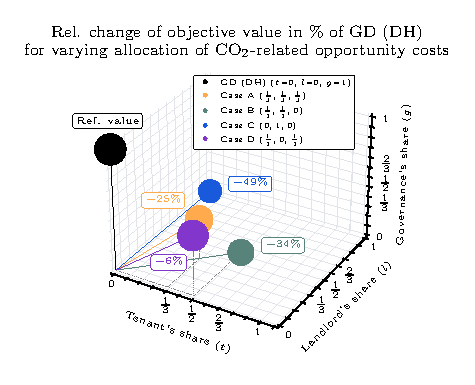
\includegraphics[width=0.75\linewidth]{figures/4_Results/fig_3d_plot/3d.eps}
	\caption{Comparison of the objective value for varying allocation of opportunity cost among the tenants (x-axis), the landlord (y-axis), and governance (z-axis) switching to district heating. The size of the points corresponds to the objective function value in proportion to the \textit{Gradual Development scenario} (percentage change in the boxes).}
	\label{fig:3dplot}
\end{figure}

Most importantly, the highest total subsidy reduction is obtained in "Case C" where the landlord has to cover the costs of inaction (-\SI{49}{\%} compared to the reference value). The second highest reduction is in "Case B". In this case, the opportunity costs are shared equally within the building among the landlord and tenants (-\SI{34}{\%}). "Case A" reduces the total subsidy by \SI{25}{\%}.  It is evident that an even allocation between the governance and the tenants ("Case D") hardly leads to a reduction of the objective value. The main reason for this is the financial support of the landlord, which is necessary to create an investment incentive, and the fact that the finacial support between the landlord and tenants necessarily has the same net present value.\vspace{0.5cm}

Eventually, Figure \ref{fig:feasible} shows the objective value for varying landlord's interest rates. Note that these results are located in the YZ-plane spanned by the landlord's and governance's share in the costs of inaction in Figure \ref{fig:3dplot}. Particularly, "Ref. value" (black, Fig. \ref{fig:3dplot}) and "Case B" (dark blue, Fig. \ref{fig:3dplot}) specify the two endpoints of the blue line in Figure \ref{fig:feasible} with $i_l=\SI{10}{\%}$. 

\begin{figure}[h]
	\centering
	\includegraphics[width=0.7\linewidth]{figures/4_Results/fig_feasible/feasible.eps}
	\caption{Comparison of the objective value for varying landlord's interest rates and share in costs of inaction}
	\label{fig:feasible}
\end{figure}

The varying landlord's interest rates have two important impacts. First, a decreasing interest rate reduces the objective value as revenues are discounted less (see Fig. \ref{fig:feasible} for a fixed landlord's share in costs of inaction, e.g., $0.2$). Second, as the interest rate decreases, a feasibility limit becomes apparent. This means, that the feasible maximum of the landlord's share in costs of inaction depends on the landlord's interest rate $i_l$ (e.g., \SI{100}{\%} for $i_l=\SI{10}{\%}$, \SI{70}{\%} for $i_l=\SI{5}{\%}$ and \SI{60}{\%} for $i_l=\SI{3}{\%}$). Two interesting energy policy implications can be derived from the results here:
\begin{itemize}
	\item In case the landlord is very much profit oriented (e.g., interest rate of $\SI{10}{\%}$) and governance's total subsidy payments are to be kept as low as possible, complete allocation of the CO\textsubscript{2}-related opportunity costs to the landlord results in a cost-optimal strategy.
	\item In contrast, in case the landlord serves rather a public-benfit purpose (e.g., interest rate of $\SI{3}{\%}$), the CO\textsubscript{2}-related opportunity costs allocation among governance, landlord, and tenants is an adequate strategy.
\end{itemize}



\section{Conclusions and recommendations}\label{conclusions}
Rapid and equitable decarbonization of the building heat sector is an indispensable cornerstone in a sustainable society. Special attention is needed for the rented residential buildings sector since a sustainable investment decision is in the landlord's hands. Simultaneously, an expected increase in the CO\textsubscript{2} price primarily impacts the tenant's energy costs. This work studies cost-optimal federal subsidy payment strategies incentivizing sustainable heat change and retrofitting measures at the multi-apartment building level. We analyze the results of a the application of the developed modeling framework to a partly renovated old building connecting to the district heating network and implementing an air-sourced heat pump system under several decarbonization storylines.\vspace{0.5cm}

We found that a fair sustainable heat system change is possible but with massive federal subsidy payments. In particular, the building's owner investment grant and additional rent-related revenues based on the building modernization are crucial to trigger the profitability of the investment. At the same time, subsidy payments are required at the beginning of the investment period to limit the energy and rent-related spendings of the tenants. Furthermore, the results imply that the heat pump alternative is not competitive in supplying heat service needs in partly renovated old buildings. Either the subsidy payments are significantly higher than in the district heating case, or the equitable constraints of the model can not be satisfied. Building renovation and reducing heat demand lead to feasibility but with high total costs because passive retrofitting measures need to be incentivized.\vspace{0.5cm}

Moreover, the results demonstrate that allocating the costs of inaction between the governance, the building owner, and the tenants is an important lever and can reduce the required subsidy payments. First and foremost, the biggest drop of the objective value (to nearly half) takes place when the costs of inaction are completely borne by the building owner. Also, a decrease in the landlord's interest rate reduces the total costs but limits the maximum share of the costs of inaction allocated to the landlord and implies a lower bound of the cost-minimized solution.\vspace{0.5cm}

Future work may investigate a stronger coupling of active and passive renovation measures as a necessary condition for federal subsidy payments. This could bring further insights to decarbonization strategies with an eye on the heat demand and sustainable heat source alternatives in the residential building sector (i.e., climate neutrality in 2050). Besides, the tenant's set-up of the building could be improved. In particular, further work should include different types of tenants within the building (e.g., different willingness to pay). More generally, this study could be extended by introducing further technology options, such as solar photovoltaic, solar thermal, and heat and electricity storage systems. 

\section*{Declaration of interests}
None.
\section*{Declaration of Competing Interest}
The authors report no declarations of interest.
\section*{Acknowledgments}
This project has received funding from the European Union's Horizon 2020 Research and Innovation Programme under Grant Agreement No. 835896. The authors acknowledge TU Wien Bibliothek for financial support through its Open Access Funding Programme.

\bibliography{mybibfile}
\appendix
\setcounter{table}{0}
\setcounter{figure}{0}
\newpage
\section{Data}\label{app:data}
Table \ref{tab:a1} shows specific emissions, energy prices, and further technical assumptions. The values correspond to the initial input parameters in $2025$ in our analysis. Furthermore, it is assumed that the specific emissions of electricity and district heating decrease linearly between $2025$ and the corresponding decarbonization target year of the scenario ($2040$ in the \textit{Directed Transition} and \textit{Societal Commitment} scenario as well as $2050$ in the \textit{Gradual Development scenario}). The energy price development of electricity, natural gas, and district heating is in line with the assumptions in \cite{fina2019profitability}. According to this, the (retail) electricity price increases by \SI{2.37}{\%} and the district heating price by \SI{5}{\%} per year. Additionally, the CO\textsubscript{2} price increases the energy price according to the specific emissions per year.

\begin{table}[h]
	\centering
	\scalebox{0.85}{
		\renewcommand{\arraystretch}{1.35}
		\begin{tabular}{llrr}
			\toprule 
			Variable & Unit & Value & Ref.\\\hline
			Specific emissions$\vert$Electricity & \SI{}{kgCO_{2} \per kWh} & \SI{0.130}{}&\cite{emissions}\\
			Specific emissions$\vert$District heating & \SI{}{kgCO_{2} \per kWh} & \SI{0.132}{}& \cite{dh_emissions}\\
			Specific emissions$\vert$Natural gas & \SI{}{kgCO_{2} \per kWh} & \SI{0.220}{}&\cite{emissions}\\
			Price$\vert$District heating & \SI{}{EUR \per kWh} & \SI{0.047}{}& \cite{dh_prices}\\
			Price$\vert$Natural gas & \SI{}{EUR \per kWh} & \SI{0.050}{}& \cite{gas_prices}\\
			Price$\vert$Electricity & \SI{}{EUR \per kWh} & \SI{0.200}{}& \cite{electricity_prices}\\
			Coefficient of performance (average) & \SI{}{1} & \SI{2.35}{}& \cite{cop_hp}\\
			\bottomrule
	\end{tabular}}
	\caption{Relevant economic parameters and further empirical settings for Austria in 2020}
	\label{tab:a1}
\end{table}
\section{Passive building retrofitting measures}\label{app:passive}
We consider passive retrofitting measures in a very simplified way in this study and focus here only on the insulation of outer wall and wall to neighboring buildings. The economic and technical assumptions are oriented to the study from Fina et al. in \cite{fina2020profitability}. Moreover, we assume the following relationships between the specific heat demand and the heat pump's (average) coefficient of performance (COP): \SI{130}{kWh \per m^2} (COP$=2.5$), \SI{115}{kWh \per m^2} ($3.0$), \SI{100}{kWh \per m^2} ($3.5$). 

\section{Empirical settings of the small case example}\label{app:verify}
\begin{table}[h]
	\centering
	\scalebox{0.85}{
		\renewcommand{\arraystretch}{1.35}
		\begin{tabular}{llr}
			\toprule 
			Variable & Unit & Value\\\hline
			Heat pump investment costs & \SI{}{EUR \per kW} & \SI{1000}{}\\
			Construction costs & \SI{}{EUR} & \SI{1000}{}\\
			Initial rent price & \SI{}{EUR \per m^2} & \SI{10}{}\\
			Rented area & \SI{}{m^2} & \SI{100}{}\\	
			Total heat demand & \SI{}{kWh} & \SI{22000}{}\\		
			Peak heat demand & \SI{}{kW} & \SI{13}{}\\	
			CO\textsubscript{2} price (2025-2034) & \SI{}{EUR \per tCO_{2}} & \SI{50}{}\\
			CO\textsubscript{2} price (2035-2040) & \SI{}{EUR \per tCO_{2}} & \SI{100}{}\\
			Natural gas price & \SI{}{EUR \per kWh} & \SI{0.05}{}\\
			Electricty price & \SI{}{EUR \per kWh} & \SI{0.2}{}\\
			Specific emissions$\vert$Electricity & \SI{}{kgCO_{2} \per kWh} & \SI{0.130}{}\\
			\bottomrule
	\end{tabular}}
	\caption{Small case example's parameters and assumptions}
	\label{tab:a2}
\end{table}

\section{Mathematical formulation for varying allocation of the costs of inaction}\label{app:varying}
This work considers the CO\textsubscript{2} price related costs as the costs of inaction and opportunity costs (OC) respectively. Hence, Equation \ref{app:eq:inaction} describes the costs of inaction per year $y$ and month $m$

\begin{align}\label{app:eq:inaction}
	OC_{y,m} =    \gamma_{init} \cdot p_{y}^{CO\textsubscript{2}} \cdot d_{y,m}
\end{align}

where $\gamma_{init}$ is the specific emissions of the initial heating system (i.e., natural gas) and $p_{y}^{CO\textsubscript{2}}$ the CO\textsubscript{2} price in year $y$ and month $m$. Exemplarily, Equation \ref{app:eq:landlord} shows the landlord's net present value in total when a part of the total OC is allocated to the landlord's net present value

\begin{align}\label{app:eq:landlord}
	OC_{l} =  \sum_{y} \sum_{m} s_l \cdot \frac{OC_{y,m}}{(1+i_l)^y} 
\end{align}

where $s_l$ is the share in the costs of inaction borne by the landlord. Consequently, Equation \ref{c:npv} is modified as follows by considering the landlord's costs of inaction.

\begin{align}\label{app:eq:landlord}
	-OC_{l} =  -\zeta + \sum_{y} \sum_{m} \frac{1}{(1+i_l)^y} \cdot \lambda_{y,m}
\end{align}

A similar logic is developed in the modification of the tenant's net present value. Therfore, the tenant's share of the costs of inaction ($OC_{t}$)are considered in Equation \ref{c:ten4}. Most importantly, the tenant's OCs influence the initial spendings that are assumed to be the limit in the sustainable heating system alternative (see Equation \ref{c:app:tenant}).

\begin{align}\label{c:app:tenant}
	K_{alt} = K_{init} - OC_{t}
\end{align}
\end{document}